% Lab Writeup for Diode-Laser Spectroscopy Lab
% Adam Reyes, George Wong
% Advanced Lab FAll 2013

%edited by adam to include methods on interferometer theory and
%discussion of broadened line spacings


\documentclass[paper=a4, fontsize=11pt]{scrartcl} % A4 paper and 11pt font size
\usepackage[left=2.5cm,top=2.5cm,right=2.5cm,bottom=2.5cm]{geometry} 
\usepackage{amsmath}
\usepackage{graphicx}
\usepackage{sectsty}
\usepackage{parskip}
\usepackage{fancyhdr}
\pagestyle{fancyplain}
\usepackage{subcaption}
\usepackage{wrapfig}
\usepackage[english]{babel}

\numberwithin{equation}{section}
\numberwithin{figure}{section} 
\numberwithin{table}{section}
%\setlength\parindent{0pt}

\fancyhead[R]{\thepage} 
\fancyhead[L]{Reyes, Wong} 
\fancyhead[C]{Saturated Absorption Spectroscopy} 
\fancyfoot[L]{} 
\fancyfoot[C]{} 
\fancyfoot[R]{} 

\newcommand{\horrule}[1]{\rule{\linewidth}{#1}}

\title{	
Saturated Absorption Spectroscopy of Rubidium
\horrule{0.5pt}
\normalfont \normalsize 
\textsc{Advanced Experimental Physics }
}

\author{Adam Reyes \\ George Wong} % Your name

\date{\normalsize\today} % Today's date or a custom date


\begin{document}
\maketitle
%%%%%%%%%Abstract%%%%%%%%%%
\noindent\textbf{Abstract:}
A diode-laser swept through the absorption bands of Rubidium was used
to measure the absorption spectrum of the Rubidium lines. With the use
of a pump beam, the saturated absorption of Rubidium was found and
used to investigate the fine structure of Rubidium. 


\section{Background}


\indent Quantum mechanics makes it well understood that an electron bound to a nucleus in
an atom is restricted to a specific set of ``allowed energies''. These energies correspond to different wavefunctions---eigenstates of the atom's energy Hamiltonian operator---that
describe the probability of finding the electron at a given point in
space. Because the energy of an electron is restricted to these specific quantities, the electron
may only absorb energy in amounts exactly equal to the differences between 
the levels. This fact is illustrated qualitatively in Figure~\ref{fig:energies}. 

 \begin{figure}[h] \begin{center}
  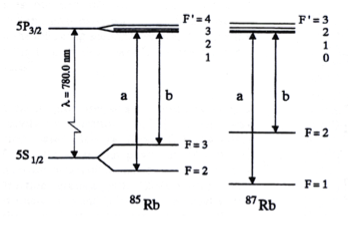
\includegraphics[height=60mm]{energy.png}
  \caption{\textbf{Energy Spectrum for Rubidium}\cite{caltech}. Horizontal lines
    represent allowed energies for a Rubidium atom. Arrows between these lines represent allowed $\Delta E$. }
  \label{fig:energies}
\end{center} \end{figure}

A photon of light carries an energy corresponding to its
frequency, given by $E_\gamma = h\nu$, where $h$ is Planck's
constant. If a photon carries energy $E_\gamma = \Delta E$, the energy
of an allowed transition for an atomic electron, then an electron can
absorb the photon and transition to a different \emph{excited} state. As the allowed $\Delta E$ form a discrete spectrum, only photons with certain frequencies can be absorbed.

Consider some source
of light, of varying frequency, incident on a sample of some atom. By measuring the intensity of the light on the far side of the sample, the absorption spectrum of the atom can be found. Because the sample will only absorb photons with particular frequencies---transmitting all others---a plot of measured intensity versus light frequency should demonstrate ``dips'' in the exiting beam intensity at the frequencies that correspond precisely
to the allowed energy transitions of the atomic electrons. A sample plot of such is given in Figure~\ref{fig:broadening}. 

\begin{figure}[h] \begin{center}
  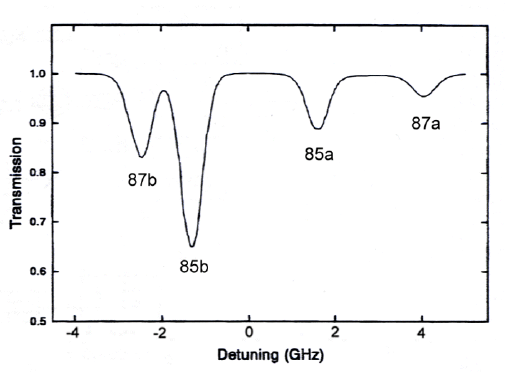
\includegraphics[height=70mm]{broadening.png}
  \caption{\textbf{Standard example of spectrum with Doppler broadening} plotting transmission intensity against  frequency offset.\cite{caltech}}
  \label{fig:broadening}
\end{center} \end{figure}


\section{Doppler Broadened Absorption}
\label{sec:broad}

\subsection{Introduction}

An notable feature of Figure~\ref{fig:broadening} is that the
absorption peaks all have some width, with absorption seemingly ``bleeding into''
frequencies around those corresponding to allowed transitions. This
phenomena is known as \textbf{Doppler Broadening}, and is a result of atoms in
the gas phase obeying a Maxwell Speed Distribution. For a light beam incident
on a sample of some gas, the velocity of the atoms in the sample will
have some component along the propagation direction of the light.

Atoms with velocity components in the direction of the light will see the light being red-shifted towards a lower
frequency, in their rest frame. Likewise in the rest frame of those atoms moving against
the incident direction of the light will see the incident light as
blue-shifted towards a higher frequency. Because of this, the sample as
a whole will absorb light of frequencies off resonance from the
frequencies associated with the allowed transitions, leading to the observed
broadened peaks of Figures~\ref{fig:broadening} and~\ref{fig:absorb1}. 

\begin{figure}[h] \begin{center}
  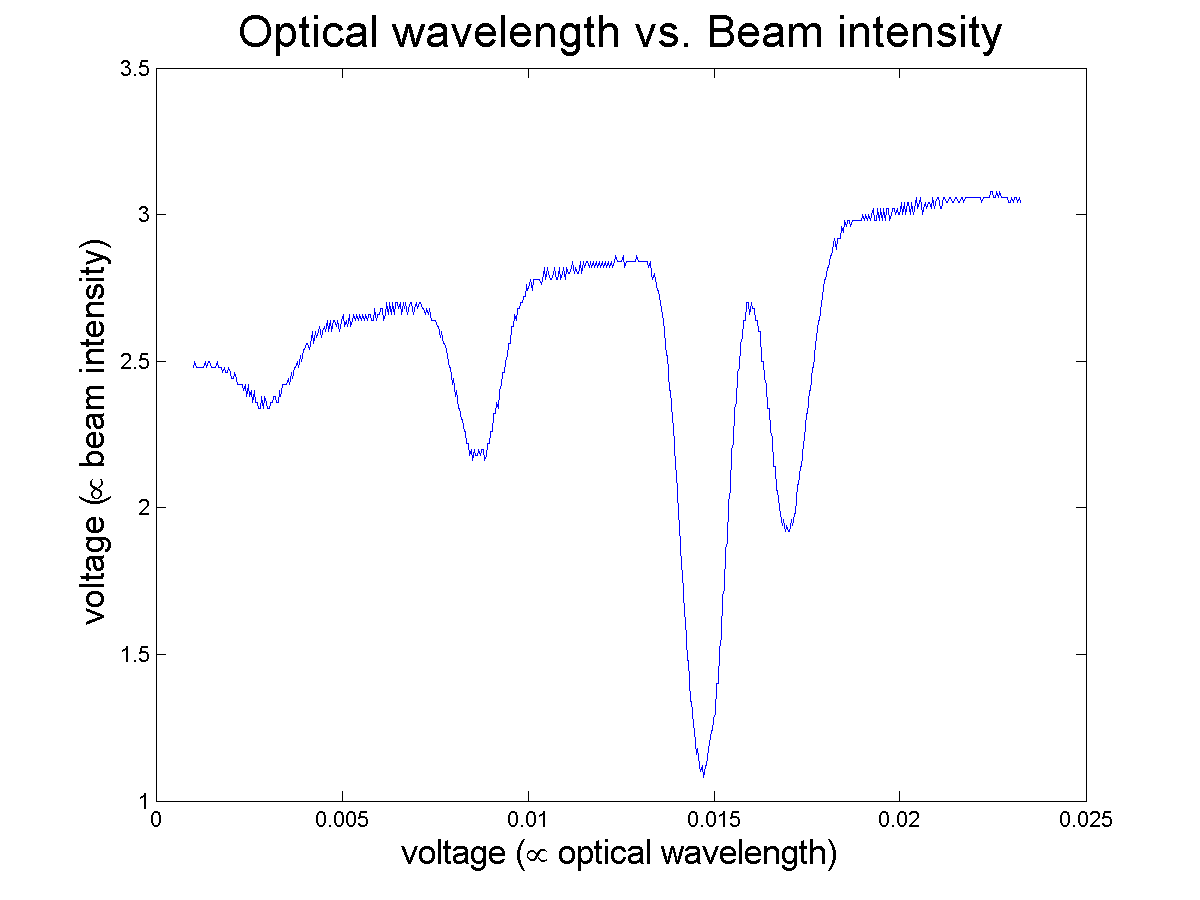
\includegraphics[height=80mm]{absorb3.png}
  \caption{\textbf{Intensity of Laser Beam with Varied Frequency through Rubidium Chamber} showing the effective absorption spectrum of Rubidium as a function of frequency (represented here as change in frequency over time). }
  \label{fig:absorb1}
\end{center} \end{figure}

\subsection{Methods}
\label{sec:dop:meth}
To observe a Doppler Broadened absorption spectrum we used a diode
laser aimed at a chamber of Rubidium gas held at $50^\circ$C. The
following steps were performed to record the absorption spectrum of Rubidium:

\begin{enumerate}
\item The laser was turned on and the current to the laser
  was increased until the beams was observed to be ``lasing''. This
  was the threshold of laser current associated with the beam, as viewed through
  the CCTV camera on a piece of paper, jumping discontinuously in intensity. 
\item The laser was aimed at and through the Rb gas chamber.
\item A ramp voltage was applied to the piezoelectric within the laser
  assembly. This voltage controlled the angle of incidence of the
  laser on a diffraction grating, effectively controlling the
  frequency of light incident on the gas chamber. 
\item A CCTV camera, capable of viewing infrared light was aimed at the Rb gas chamber. The incident current to the laser assembly was increased until florescence was seen.
\item A photoelectric diode, capable of reporting incoming light
  intensity in the form of voltage, was placed in the path of the beam
  exiting the Rubidium chamber.
\item The voltage from the diode was measured on an oscilloscope
  against ramp voltage to the piezo ($\propto$ frequency of light).
\item The voltage offset, frequency, and slope of the ramp were adjusted, as was the current to the laser. This was done until the absorption spectrum of both the $^{85}$Rb and $^{87}$Rb isotopes could be seen on the scope.
\item Several samples of the spectrum were taken. They are reproduced in Figures~\ref{fig:absorb1}$-$\ref{fig:absorb2}.
\item The voltage from the diode was then subtracted from the voltage of the ramp, with the scales of the two appropriately adjusted for compatibility. This allowed for observation of the spectrum without the ramp voltage artifact.
\end{enumerate}

\subsection{Results}

Figures~\ref{fig:absorb1} and~\ref{fig:absorb2} show the absorption spectrum recorded during the first part of the experiment. Doppler broadening is evident, as is noise in the signal.

\begin{figure}[h] \begin{center}
  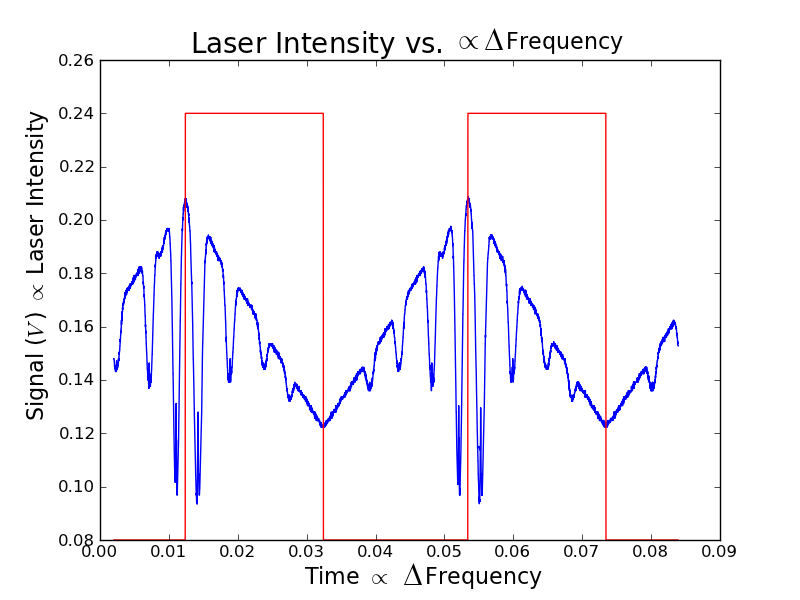
\includegraphics[height=80mm]{2-2-002.png}
  \caption{\textbf{Intensity of Laser Beam vs. Varying Laser Frequency
      with Pump} shown over the course of approximately two full
    cycles in frequency. The red lines show the beginning and end of
    one ramp cycle.}
  \label{fig:absorb2}
\end{center} \end{figure}

\section{Michelson Interferometer}

\subsection{Introduction}

In order to numerically interpret a recorded absorption spectrum, knowledge of the frequency (or relative frequency) of the light incident on the sample is essential. Since the diffraction grating sweeps through its position
at a constant rate, a Michelson Interferometer can be set up and used to relate the time dimension of the oscilloscope traces to a relative frequency scale. With this relation, the difference in frequencies between excited and ground states of the Rubidium spectrum may be measured.

A Michelson Interferometer is constructed by splitting a beam of light
into two ``arms'' with a difference in path length distance, denoted $\Delta L$. The light is recombined and sent into a detector. The difference in path length results in the recombined beams being out of phase, thereby effecting interference. The combined beam's intensity will go as given in Equation~\ref{eq:intensity-interferometer}
\begin{equation}
\label{eq:intensity-interferometer}
I \propto 1 + \cos \frac{4\pi \Delta Lf}{c}
\end{equation}
where $f$ is the frequency of light and $c$ is the speed of light. If
the frequency of the light is shifted, then the intensity will go sinusoidally, with period given by Equation~\ref{eqn:T} where $\Delta f$ corresponds to change in frequency.
\begin{equation}
\label{eqn:T}
T = \frac{2\Delta L \Delta f}{c}
\end{equation}

 Equation~\ref{eqn:T} can be inverted to give $\Delta f$, as in Equation~\ref{eqn:df}.
\begin{equation}
\label{eqn:df}
\Delta f = \frac{c}{2\Delta L T}
\end{equation}

\subsection{Methods}

The same laser with tuning from Section~\ref{sec:broad} (to show the absorption spectrum of Rubidium) was used. A diagram of the
interferometer can be found in Figure~\ref{fig:setup} as the part of
the apparatus beginning with the reflected beam from the first beam splitter. The following steps were performed to set up the apparatus:
\begin{enumerate}
\item The beam incident to the wedge was split into two (using a beam splitter) and the stronger beam was sent to the interferometer (setup described below).
\item The interferometer beam was sent to a $50-50$ beam splitter placed at an angle to ``create'' a new beam perpendicular to the incident one.
\item In the path of the original beam was placed a mirror which reflected light back at the beam splitter.
\item In the path of the new beam (leaving the splitter at $90^\circ$
  to the original beam) was placed another mirror. This mirror
  reflected the beam back to the splitter. This mirror was placed as
  far away from the splitter as possible, so as to maximize the
  difference in distance both beams (original and split) traveled. A path length difference of $\Delta L=1.7971 \pm 0.0001$m was measured.
\item The two beams (off of both mirrors) were aligned after passing through the beam splitter one last time.
\item This aligned beam was directed into a photoelectric diode to measure light intensity.
%\item Measurements of absorption spectra (with pump beam to point out hyperfine splitting) were made alongside interferometer intensity. Figure~\ref{fig:int_1} represents these data.
\end{enumerate}

\subsection{Results}

\begin{figure}[h] \begin{center}
  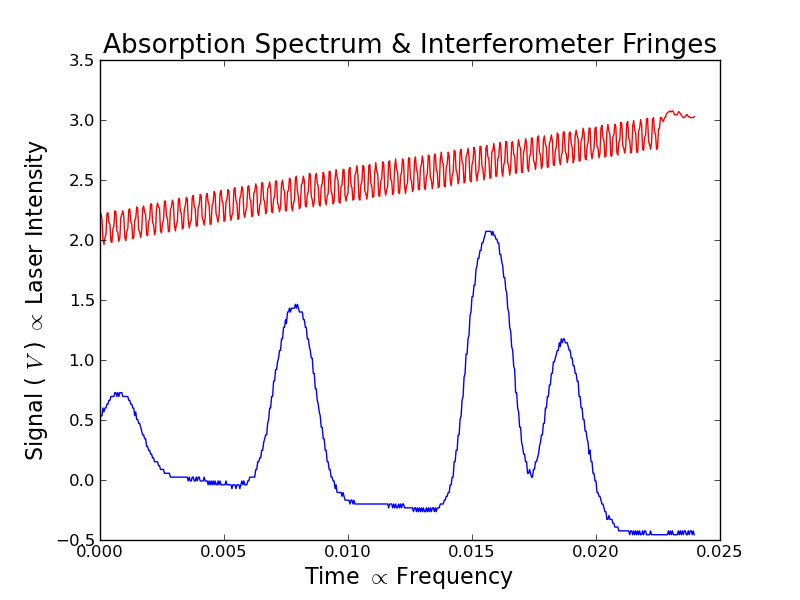
\includegraphics[height=70mm]{4-1-009.png}
  \caption{\textbf{Laser Intensity \& Interferometer Beam Intensity over Change in Frequency} demonstrating the changing intensity (fringes) generated by the interferometer over the same interval as the intensity incident from the laser beam traveling through the Rubidium chamber. }
  \label{fig:int_1}
\end{center} \end{figure}

Figure~\ref{fig:int_1} shows the interference patter (in red)
alongside the Rubidium absorption spectrum. To establish a relation between time and frequency, the number of periods in a given interval of
the interference pattern were counted. Using Equation~\ref{eqn:df}, $\frac{\Delta f}{T}$ can be calculated to give a conversion
between time and frequency. A $\frac{\Delta f}{T} = 0.004 \pm
.002\frac{\normalfont{GHz}}{\normalfont{ms}}$ was found. Figure~\ref{fig:detuning}
shows the absorption spectrum of Rubidium against the detuning (frequency offset) from
the largest peak. 

The error here is dominated by the determination of $\Delta L$ and
could be reduced by increasing the path length difference between the two arms of the interferometer. Because of the fixed length of the BNC
cables, however, there was a limit of roughly half the length of the optics bench for the long arm.  

\begin{figure}[h] \begin{center}
  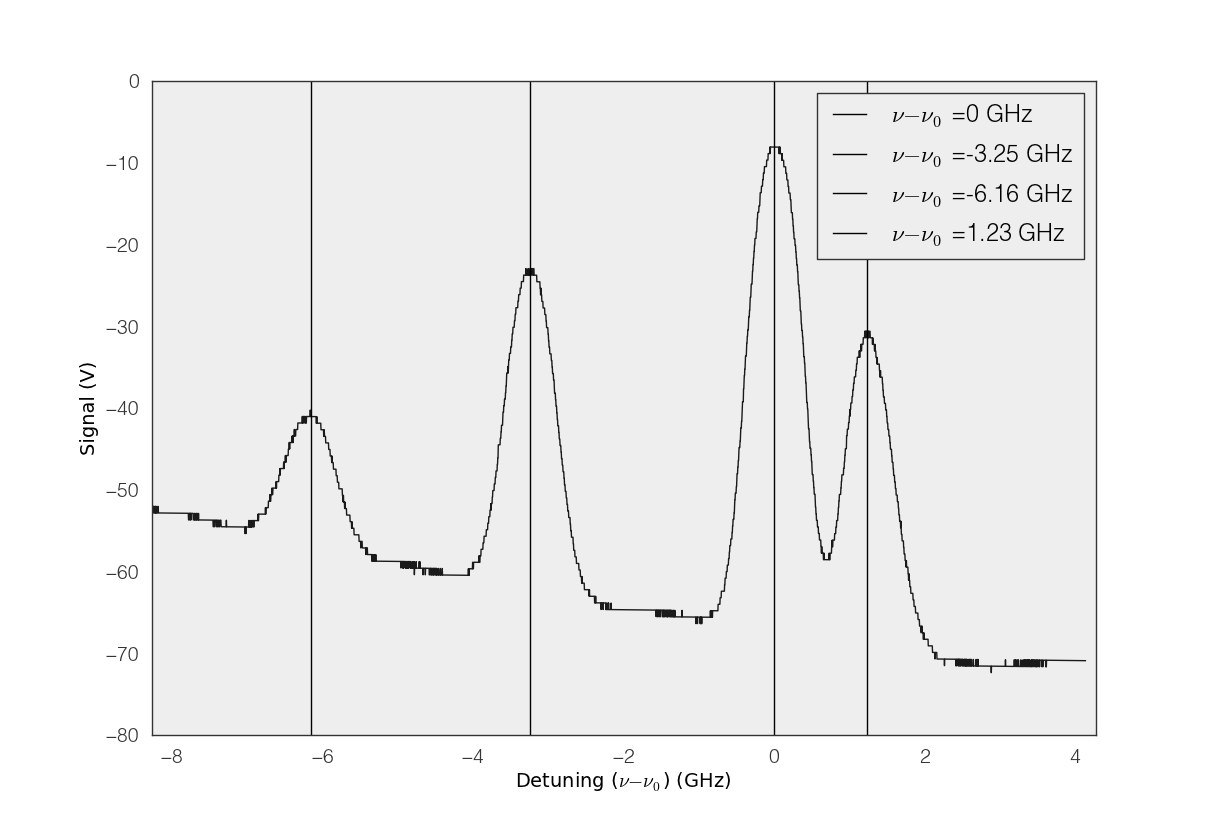
\includegraphics[height=80mm]{Detuning.png}
  \caption{\textbf{Absorption Spectrum of Rubidium } with
      interferometrically determined detuning centered about the largest peak. }
  \label{fig:detuning}
\end{center} \end{figure}

\begin{table}[h]
\centering
\caption{Average frequency difference ($\Delta$GHz) between peaks with associated error}
\begin{tabular}{ || c | c c c c || }
  \hline
  \hline
   $-$ & 87a & 85a & 85b & 87b \\
  \hline
  87a & $-$ & $2.91 \pm 0.08$ & $6.16 \pm 0.13$ & $7.39 \pm 0.17$ \\
  85a & $2.91 \pm 0.08$ & $-$ & $3.25 \pm 0.11$ & $4.48 \pm 0.16$ \\
  85b & $6.16 \pm 0.13$ & $3.25 \pm 0.11$ & $-$ &  $1.23 \pm 0.07$ \\
  87b & $7.39 \pm 0.17$ & $4.48 \pm 0.16$ & $1.23 \pm 0.07$ & $-$  \\
  \hline
  \hline
\end{tabular}
\label{table:freqOffset}
\end{table}

Table~\ref{table:freqOffset} has the values for the detuning between
the various absorption peaks, so labeled in Figure~\ref{fig:detuning},
and averaged over several data sets. Accepted values place the spacing between $^{87}$Rb lines at $6.8$ GHz, and spacing between $^{85}$Rb lines at $3.035$ GHz. These values are somewhat comparable (though not entirely so) with the measured averaged measured spectrum produced in this experiment.

\clearpage
\begin{figure*}[h]
  \centering
  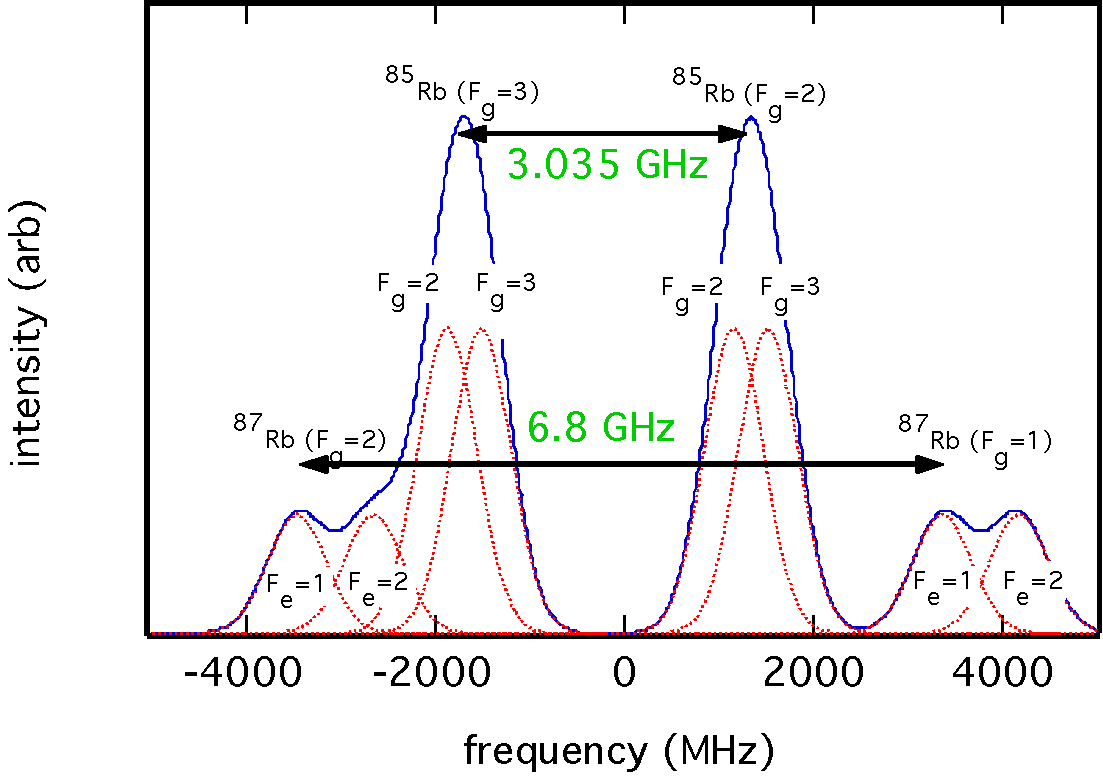
\includegraphics[width=3in]{/Users/adamreyes/Dropbox/AdvancedLab/Diode-Laser-Spec/WriteUp/figures_laserspec/fluorescence.png}
  \caption{Literature Values for the Rubidium absorption lines\cite{vanier}\cite{harvard}}
  \label{fig:literature}
\end{figure*}



\section{Saturated Absorption}

\subsection{Introduction}
\label{sec:satabintro}
Figure~\ref{fig:energies} shows that the 5P$_{\frac{3}{2}}$
ground state of both Rubidium isotopes is split into two levels, given by the F' quantum
number. This splitting is due to coupling of the electron's spin to
its orbit and is called the hyperfine structure. 

It may be noticed, however, that in the absorption spectra so far discussed
(Figures~\ref{fig:absorb1} and~\ref{fig:broadening}), only
the wide Doppler broadened lines expected for the un-split
5P$_{\frac{3}{2}}$ state can be seen. This is because, as shown in Figure~\ref{fig:energies}, the 5P$_{\frac{3}{2}}$ splittings are much
more closely spaced than the ground state lines and--more importantly--closer together than the Doppler broadening for each
transition. Because the Doppler broadening is wider than the
separation of the excited state splittings, the hyperfine structure cannot be seen in a
regular absorption experiment.

To overcome this issue of resolution, a refined setup is used. Consider two collinear beams incident on the
Rubidium sample coming from opposite directions. One beam is given a far greater intensity than the other. The weaker
beam is called the \emph{probe} beam and the beam with the greater intensity is called the \emph{pump} beam. It is the intensity of the probe beam that is measured after it exits the Rubidium gas.

Atoms in the sample with a velocity component parallel (or anti-parallel) to the direction of the beam will be shifted in opposite frequency directions. As before, this results in typical Doppler broadening off-resonance (with respect to the transitions). For atoms with zero velocity component in the propagation direction, however, there is no frequency shift for \emph{either} beam, thus both beams are absorbed. Because the pump beam is so intense, these atoms will be saturated, preventing the probe beam from being absorbed. Thus, when the probe beam is on resonance, there will be a higher transmission percentage, allowing the file structure of the Rubidium spectrum to be observed.

Another consequence of the close frequency proximity of the split
5P$_{\frac{3}{2}}$ states is the phenomena of cross-over
peaks. Consider two closely spaced resonant lines at frequencies
$\nu_1$ and $\nu_2$ and a light frequency of $\nu_{\gamma} = \frac{\nu_1 +
  \nu_2}{2}$. Because of Doppler broadening, there will be a ``false''
peak at $\nu_{\gamma}$. 


\subsection{Methods}
\label{sec:satabmeth}
\begin{figure}[h] \begin{center}
  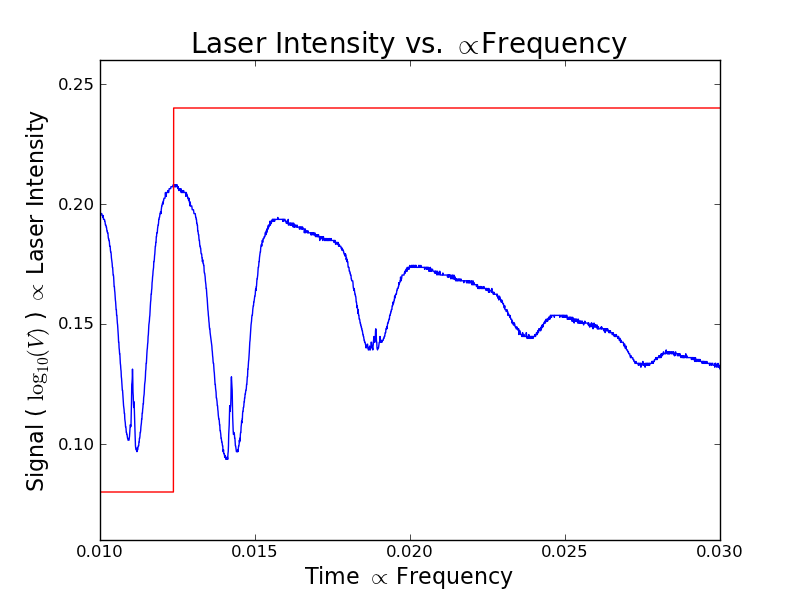
\includegraphics[height=75mm]{2-2-002-zoom.png}
  \caption{\textbf{Intensity of Laser Beam vs. Varying Laser Frequency with Pump} shown over a restricted interval. A Pump beam has clearly been added, as hyperfine splitting is more easily observable. }
  \label{fig:withPump_1}
\end{center} \end{figure}
The same Rubidium cell and laser from Sec.~\ref{sec:dop:meth} were
used in this experiment. A diagram of our apparatus is shown in Figure
~\ref{fig:setup}. The following steps were carried out in performing
this experiment. 
\begin{enumerate}
\item Instead of being reflected by a mirror directly into the
  chamber, the laser beam was sent into a 2$^\circ$ wedge. The two reflected beams were sent
  into the Rubidium chamber and into two photo-diode detectors on the
  other side.
\item The beam transmitted by the wedge was reflected around the chamber by using mirrors. This beam was to be the pump beam.
\item The pump beam was aimed at a 50-50 beam
  splitter that reflected it into the chamber.
\item The pump beam was then aligned to be collinear with one of the
  beams coming from the wedge (probe beam). The probe beam intensity was
  plotted as shown in Figures~\ref{fig:satabsorb1} and~\ref{fig:withPump_1}
\item The signal from the probe beam was subtracted electronically
  from the reference signal coming from other wedged beam as shown in Figure~\ref{fig:scaled_1}. 
\end{enumerate}

\clearpage
\begin{figure}[h] \begin{center}
  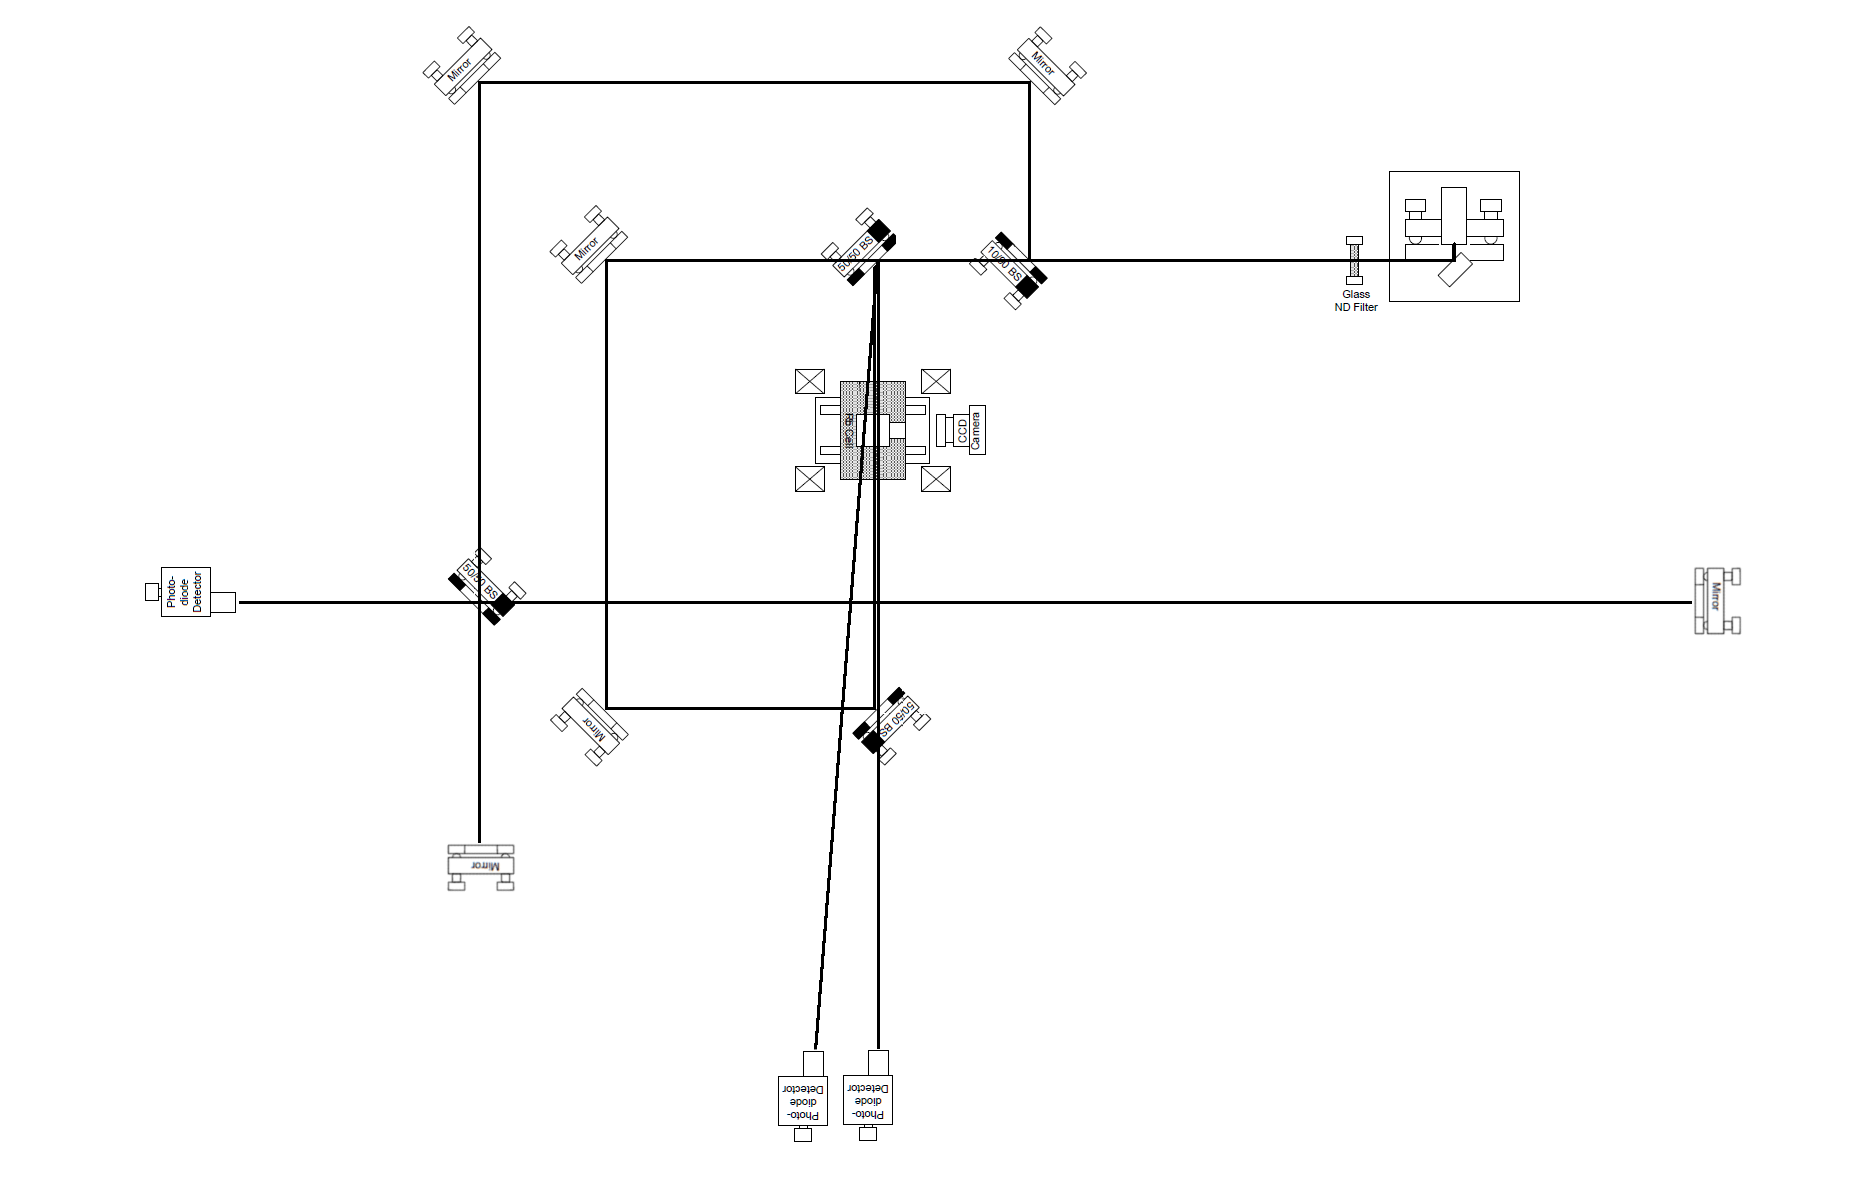
\includegraphics[height=6in, angle = 0]{full.png}
  \caption{\textbf{Overall final set up of apparatus} showing
    placement of all beam splitters, mirrors, and various other
    devices to simultaneously measure the saturated absorption
    spectrum and take interferometric measurements. }
  \label{fig:setup}
\end{center} \end{figure}
\clearpage

\begin{figure}[h] \begin{center}
  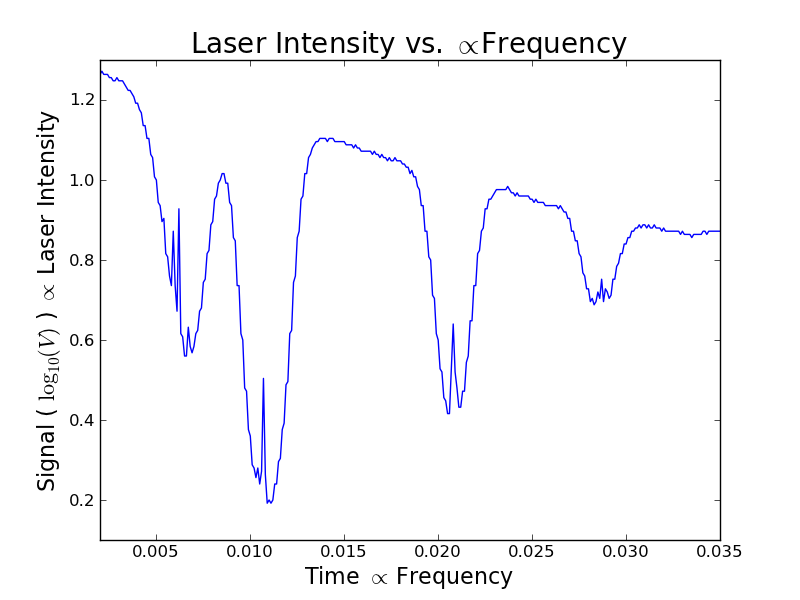
\includegraphics[height=100mm]{3-1-001.png}
  \caption{\textbf{Hyperfine splitting} as observed with the experimental set up used for this examination (sample shows intensity from combination of pump and probe beams). }
  \label{fig:satabsorb1}
\end{center} \end{figure}

% \begin{figure}[h] \begin{center}
%   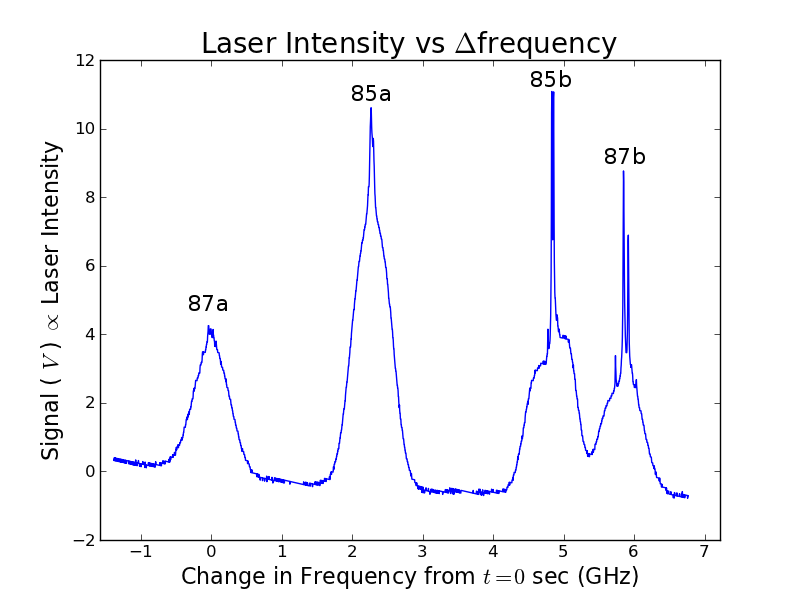
\includegraphics[height=70mm]{4-2-009.png}
%   \caption{Saturated absorption \textbf{Plot of intensity vs. frequency shift} for data sample 1. }
%   \label{fig:scaled_1}
% \end{center} \end{figure}

\subsection{Results}

%%%%%%%%HERE GOES TABLES AND STUFF FROM OTHER DRAFT%%%%%%%%%%%%%%%%%%%%%%%

Figures~\ref{fig:scaled_1}$-$\ref{fig:scaled_4} show four data samples
illustrating hyperfine splitting plotted against frequency shift. In
each of the plots, the first peak (corresponding to the 87a
absorption) is denoted as the $\Delta 0.00$ GHz point. All detuning is
centered around this peak. Values given on
Tables~\ref{table:relativePositions87}
and~\ref{table:relativePositions85} show the spacing between nearby
fine structure lines. Values given on these two tables were estimated, and in the case where an exact value was indeterminable, the field was left blank. Random error exists here both due to the time resolution with which the samples were taken and the human estimation.

\begin{figure}[h] \begin{center}
  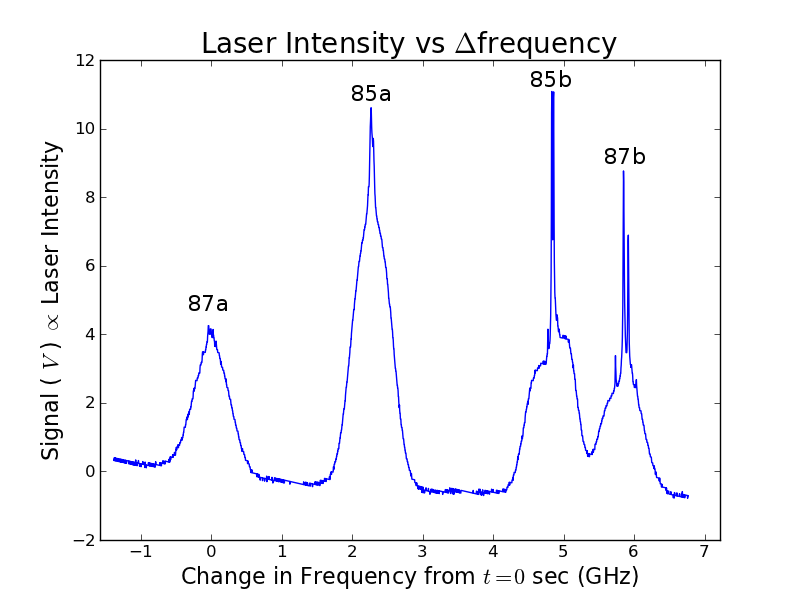
\includegraphics[height=70mm]{4-2-009.png}
  \caption{Saturated absorption \textbf{Plot of intensity vs. frequency shift} for data sample 1. }
  \label{fig:scaled_1}
\end{center} \end{figure}

\begin{figure}[h] \begin{center}
  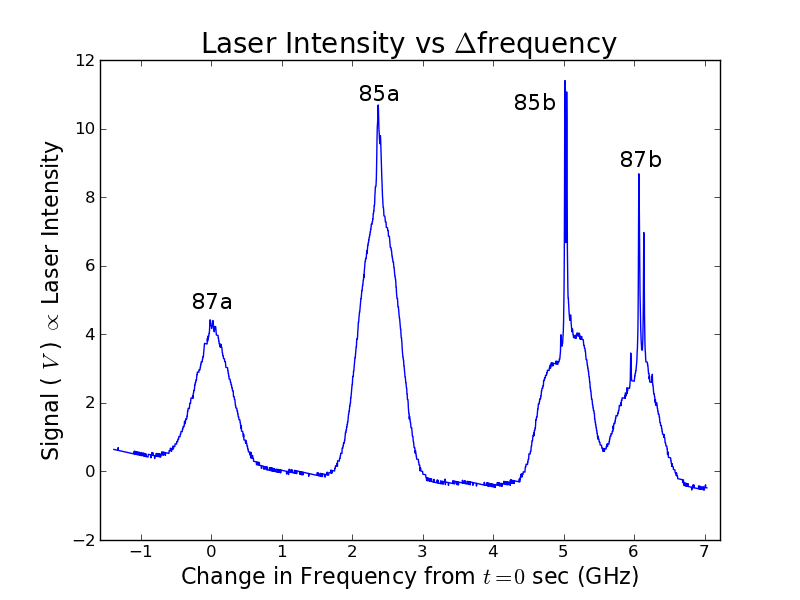
\includegraphics[height=60mm]{4-2-010.png}
  \caption{Saturated absorption \textbf{Plot of intensity vs. frequency shift} for data sample 2. }
  \label{fig:scaled_2}
\end{center} \end{figure}

\begin{figure}[h] \begin{center}
  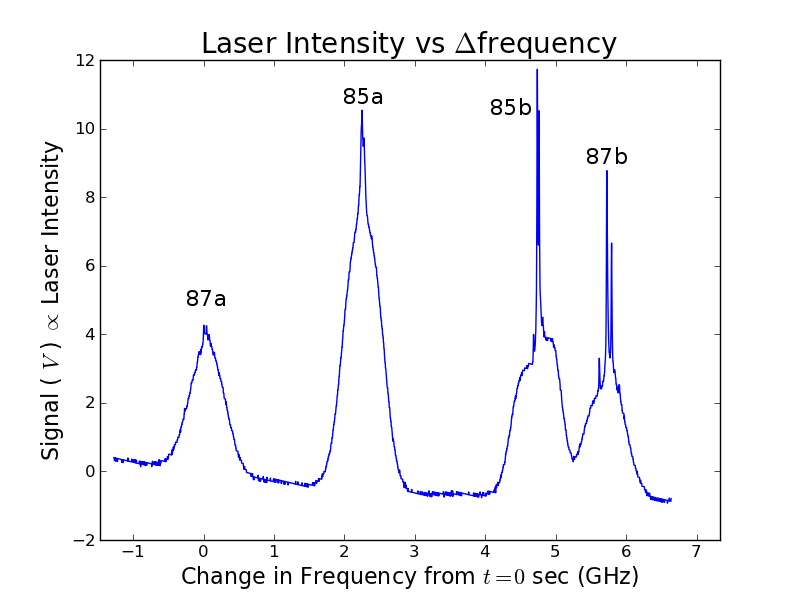
\includegraphics[height=60mm]{4-2-011.png}
  \caption{Saturated absorption \textbf{Plot of intensity vs. frequency shift} for data sample 3. }
  \label{fig:scaled_3}
\end{center} \end{figure}

\begin{figure}[h] \begin{center}
  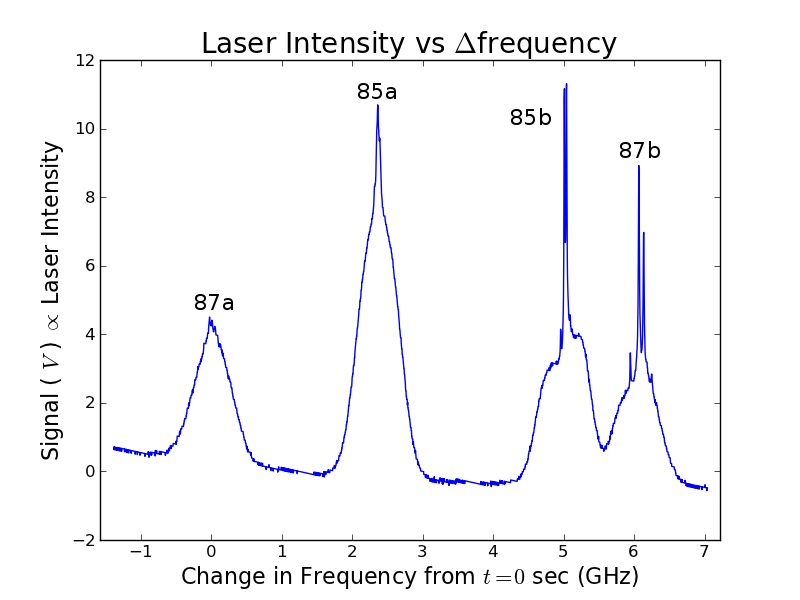
\includegraphics[height=60mm]{4-2-012.png}
  \caption{Saturated absorption \textbf{Plot of intensity vs. frequency shift}  for data sample 4. }
  \label{fig:scaled_4}
\end{center} \end{figure}

\begin{table}[h]
\centering
\caption{Relative positions of peaks (in GHz) for $^{87}$Rb, with values given to $\pm 0.05$ GHz}
\begin{tabular}{ c | c c c c | c c c c }
  \hline
  \hline
  sample no. & a & & & & b   \\
  \hline
  1 & $-$ & $-$ & $-$ & $-$ & 5.97 & 6.09 & 6.16 & 6.27 \\
  2 & 0.00 & 0.04 & 0.08 & $-$ & 5.97 & 6.09 & 6.16 & 6.28 \\
  3 & 0.00 & 0.04 & $-$ & $-$ & 5.62 & 5.73 & 5.79 & 5.83  \\
  4 & 0.00 & 0.03 & 0.07 & $-$ & 5.97 & 6.09 & 6.17 & 6.28
\end{tabular}
\label{table:relativePositions87}
\end{table}

\begin{table}[h]
\centering
\caption{Relative positions of peaks (in GHz) for $^{85}$Rb, with values given to $\pm 0.05$ GHz}
\begin{tabular}{ c | c c c c | c c c c | c c c c | c c c c }
  \hline
  \hline
  sample no. & a & & & & b  \\
  \hline
  1 & 2.5 & 2.53 & $-$ & $-$ & 5.01 & 5.07 & 5.10 & 5.15 \\
  2 & 2.39 & 2.42 & $-$ & $-$ & 4.98 & 5.04 & 5.06 & 5.12 \\
  3 & 2.25 & 2.27 & $-$ & $-$ & 4.68 & 4.74 & 4.76 & 4.81 \\
  4 & 2.34 & 2.39 & 2.42 & $-$ & 4.99 & 5.04 & 5.07 & 5.12 
\end{tabular}
\label{table:relativePositions85}
\end{table}






\begin{figure}[h] \begin{center}
  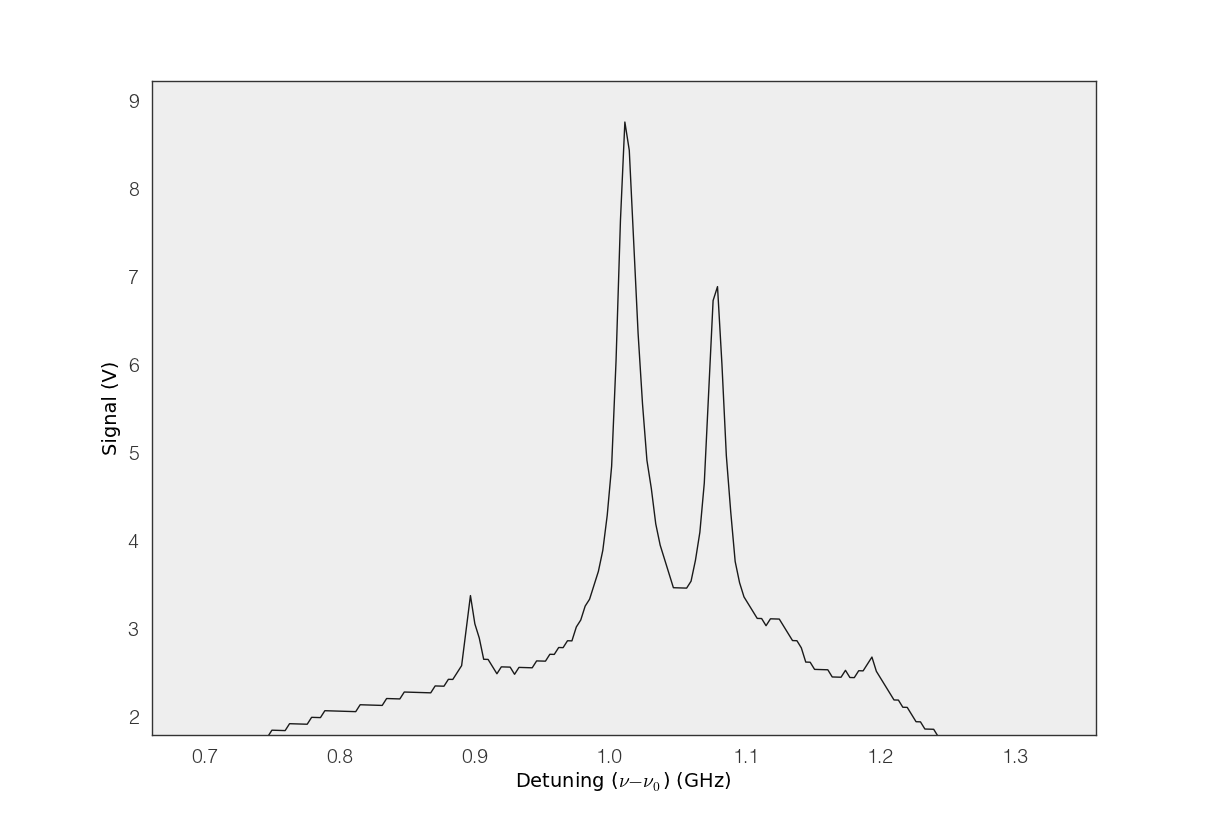
\includegraphics[height=70mm]{detune1.png}
  \caption{Saturated absorption \textbf{Plot of intensity
      vs. detuning} from $^{85}$Rb b line in
    Figure~\ref{fig:scaled_1}, zoomed in to show fine structure. 87b
    line shown here.}
  \label{fig:det1}
\end{center} \end{figure}

\begin{figure}[h] \begin{center}
  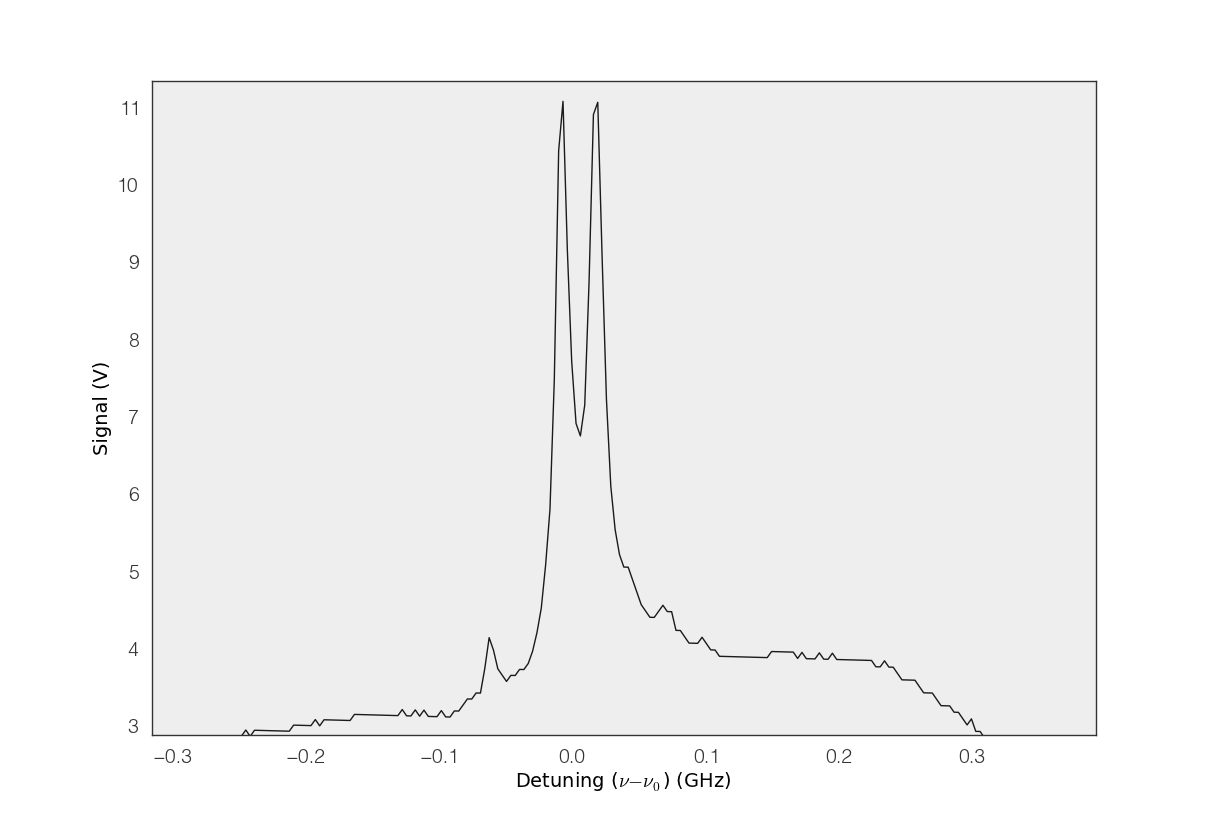
\includegraphics[height=70mm]{detune2.png}
  \caption{Saturated absorption \textbf{Plot of intensity vs. detuning} from $^{85}$Rb b line in
    Figure~\ref{fig:scaled_1}, zoomed in to show fine structure. 85b
    line shown here.}
  \label{fig:det2}
\end{center} \end{figure}

It would be expected to see evidence of crossover peaks in
Figures~\ref{fig:det1} and~\ref{fig:det2}, which show a blown-up
views of the $87$b and $85$b lines (see Figure~\ref{fig:scaled_1} for relative locations). In both plots, two well-defined peaks of large amplitude can be seen. In Figure~\ref{fig:det1}, two smaller peaks can be seen at around $0.9$ and $1.2$ GHz. Another candidate for a peak can be seen at $\approx 1.1$ GHz. In the 85b spectrum (Figure~\ref{fig:det2}), again two peaks
with large amplitude and two smaller peaks at around $\pm$ 0.8 GHz
detuning can be seen.

From Figure~\ref{fig:energies}, it is shown that both $^{85}$Rb and $^{87}$Rb have are split into four energy levels in their excited state. As noted above, at least four peaks are observed. A fifth peak would be persuasive evidence of one peak being a cross-over peak.

Due to the fact that a cross-over peak would have contributions from multiple excited state transitions, it would be expected that they would have greater intensity than the regular resonance peaks. This seemingly contradicts the data, as the odd peak of the five has a lower intensity (indicating either two cross-over peaks and only three resonance peaks, or one cross-over peak of lesser amplitude).

As can be seen in the Doppler-subtracted spectrum
(Figure~\ref{fig:scaled_1}), the resulting spectrum is not ideal. There was great difficulty in finding the right combination of the two
signals to exactly subtract the Doppler broadening, and so if the
missing peaks were of small enough amplitude it is reasonable that
they might have been lost completely in the process.

As with all alignment procedures, it was incredibly difficult to align the pump and probe beams so that they collectively resulted in a spectrum that highlighted the hyperfine splitting.


\section{Resonant Absorption}
\label{sec:resab}


Because there was extra time available at the end of the experiment, we decided to attempt to observe the relation between resonant absorption and the refractive index in Rb gas.

To do so, we took one incident beam, split it in two, passed one through the Rb chamber, and had the other travel the same distance, but not pass through the chamber. The two beams were then recombined and this sum (with interference) was then passed into a photoelectric diode. Changes in frequency between the two beams (frequency change due to refractive index of Rb gas) should effect interference which should be measurable with the diode.

Unfortunately, we were unable to precisely reproduce this effect. We attempted aligning the two beams multiple ways; however, we never were able to see evidence of interference, or if we did, it was too faint to be in any way noticeable.
% NOTE ABOVE THAT "EFFECT" with an "E" is the right word to use. I know the verb is normally "Affect", but in this case it's "effect". Not to be rude, just /so many people/ get this wrong because they learn that an "effect" is only ever a noun.

\clearpage
\begin{thebibliography}{99}
\bibitem{vanier}Jacques Vanier. Relaxation in rubidium-87 and the
  rubidium maser. Phys. Rev., 168:129-149, 1968.
\bibitem{harvard}"Rubidium Fluoresence." Cfa.harvard.edu. Harvard,
  n.d. Web.
\bibitem{caltech}Caltech Department of Physics. Saturated Absorption
Spectroscopy. Caltech
\end{thebibliography}


%%%%%%%%%%%FIGURES%%%%%%%%%%%%


\end{document}
